\section{LC-Modulator als DOE}
\subsection{Berechnung der Pixelgröße}
\subsubsection{Theorie}
Zur Bestimmung der Breite eines Pixels innerhalb des LC-Modulators wird mit der Formel eines Gitters gerechnet, da ein LC-Modulator dasselbe Beugungsbild aufweißt.
\begin{align}
	g\sin{\alpha} = m\lambda
	\label{gbestimm}
\end{align}
Dabei stellt g die Gitterkonstante, $\alpha$ den Winkel zwischen der nullten und m.ten Beugungsordnungen, m die entsprechende Beugungsordnung und $\lambda$ die Wellenlänge des Lasers ($\lambda = 650nm$) dar.
Die Bestimmung von $\alpha$ kann aus der Optik durch
\begin{align}
	\alpha \approx \frac{d}{2f}
	\label{abestimm}
\end{align}
berechnet werden. Dabei ist d der Abstand zweier gleicher höherer Ordnungen. 
\subsubsection{Aufbau}
Der Aufbau zur Berechnung der Pixelgröße ist in \cref{421} dargestellt.
Zuerst wird der Laser auf einen LC-Modulator gerichtet, welcher in dem Abstand der Brennweite der Linse ($f = 16cm$) von der Linse entfernt steht. Zwischen der Linse und dem LC-Modulator ist ein Analysator. Hinter der Linse ist im Abstand ihrer Brennweite ein Schirm aufgestellt, um die Beugungsordnungen messen zu können. 
\begin{figure}[h!]
	\centering
	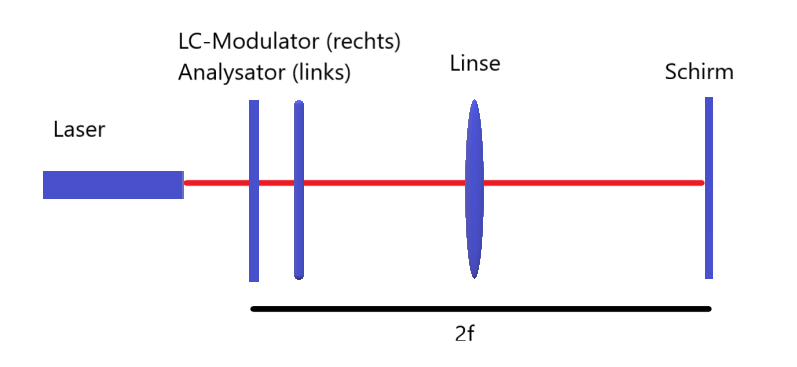
\includegraphics[scale = 1]{4.2.1-Aufbau.png}
	\caption{Aufbau zur Bestimmung der Pixelgröße}
	\label{421}
\end{figure}
\subsubsection{Auswertung}
Um \cref{gbestimm} möglichst genau zu berechnen wurde bei der Berechnung von \cref{abestimm} der Abstand der siebten Ordnungen benutzt, um d zu messen. Dieser Abstand wurde mittels eines Lineals gemessen. Aus diesen Berechnungen kann die Gitterkonstante bestimmt werden $g = (29 \pm 3) \mu m$.
\subsubsection{Unsicherheiten}
Die Unsicherheit von d wurde mit einer Genauigkeit von $\pm 0,2cm$ angenommen. Daraus resultiert für die Unsicherheit der Gitterkonstanten mittels Fehlerfortpflanzung ein Wert von $g = (29 \pm 3) \mu m$.
\subsubsection{Diskussion}
Somit liegt das Ergebnis der Pixelgröße innerhalb der angegebenen Pixelgröße von $g = 32 \mu m$.
Die Diskussion mit dem Aufgabenteil 1 muss auch noch geschrieben werden.

\subsection{Intensitätsverteilung in den Beugungsordnungen des unadressierten Displays}
\subsubsection{Theorie}
Eine LCD-Zelle besitzt eine Untermodulation. Dies ist deshalb der Fall, da in einem einfachen Pixel es einen transparenten Anteil gibt, sowie einen Lichtundurchlässigen Anteil. Die Modulation wird durch das Gitter beschrieben, welches im vorherigen Aufgabenteil behandelt wurde. Die Untermodulation wird durch die Substruktur im Pixel erzeugt. An dieser Stelle wird der duty cycle definiert. Dieser beschreibt das Verhältnis zwischen transparentem und lichtundurchlässigem Teil. 
Dieser wird berechnet, indem sinc-Funktionen an die Untermodulation angepasst werden. Die Breiten der sinc-Funktionen entsprechen dann dem durchlässigen Anteil in der jeweiligen Richtung. 
Der duty cycle ergibt sich dann durch
\begin{align}
	duty cycle = \frac{xy}{g^{2}-xy}
	\label{dutycyc}
\end{align}
Ebenfalls kann auf den Füllfaktor geschlossen werden für den transparenten Teil des Pixels. Dieser entspricht gerade dem Anteil des durchlässigen Pixels zur Gesamtpixelgröße.
\begin{align}
	FF = \frac{xy}{g^{2}}
	\label{ff}
\end{align}

\subsubsection{Aufbau}
Der Aufbau zur Berechnung des Füllfaktors der LCD-Zelle ist in \cref{422} dargestellt. Zuerst wird der Laser, welcher eine zusätzlich integrierte Aufweitungsoptik besitzt auf das LCD-Display gerichtet. Danach wird ein Analysator in den Strahlengang geführt. Statt einem Schirm wird die Auswertung mit einem Intensitätsmessgerät durchgeführt.
\begin{figure}[h!]
	\centering
	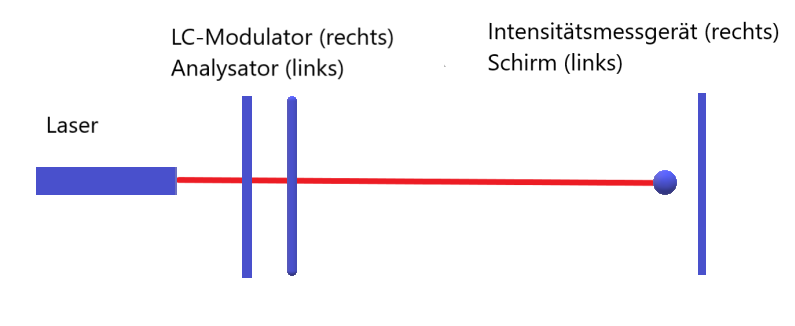
\includegraphics[scale = 1]{4.2.2-Aufbau.png}
	\caption{Aufbau zur Bestimmung des Füllfaktors der LCD-Zellen}
	\label{422}
\end{figure}
\subsubsection{Auswertung}
Im weiteren wurden die ersten zehn Beugungsordnungen in horizontaler und vertikaler Ebene gemessen. Die Messwerte sind in \cref{horiz} zu sehen.
\begin{figure}[h!]
	\centering
	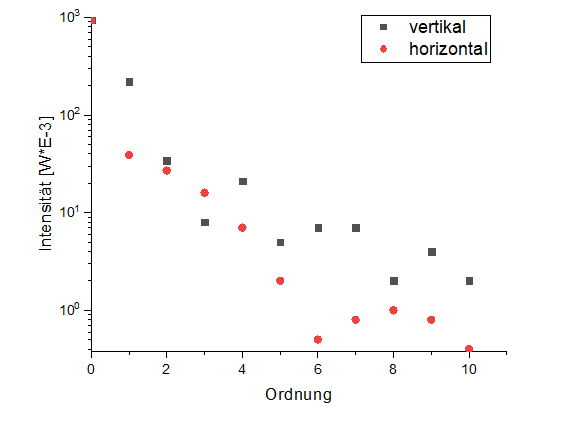
\includegraphics[scale = 1]{horizundvertik.png}
	\caption{Intensitätsverteilung der horizonatlen und vertikalen Beugungsordnungen}
	\label{horiz}
\end{figure}
Aus den Messwerten kann auf den duty cycle geschlossen werden, sowie auf den Füllfaktor des transparaneten Teils der LCD-Zelle in Bezug auf das Gesamte Pixel. Um den duty cycle zu berechnen wird \cref{dutycyc} benutzt. Hierfür werden die Breiten der sinc-Funktionen nicht durch den Fit bestimmt, welcher Aufgrund der wenigen Messdaten nicht funktioniert hat, sondern es wird visuell das Minimum der sinc-Funktionen gesucht und damit den Stauch- bzw. Streckfaktor innerhalb der sinc-Funktion berechnet. Über einen Vergleich des Stauchfaktors kann die Breite des Peaks entnommen werden.
Daraus ergibt sich ein duty cycle und ein Füllfaktor von 
\begin{align}
	\text{duty cycle} = (5 \pm 0,4)\% \\
	\text{Füllfaktor} = (4,7 \pm 0,3)\%
\end{align}
\section{Unsicherheiten}
Die Unsicherheiten wurden durch die oben genanten Unsicherheitsannahmen mittels Fehlerfortpflanzung berechnet.
\section{Diskussion}
Der Füllfaktor, welcher durch die obige Auswertung berechnet wurde, ist nicht gleich mit der Angabe des Herstellers, welcher in [1] aufgelistet wurde. In den Angaben des Herstellers ist der geringste Füllfaktor bei einem Wert von $58 \%$. Der oben ausgerechnete Wert unterscheidet sich in einer Zehnerpotenz von dem Soll Wert. Hingegen ist die Pixelbreite von $g = (29 \pm 3) \mu m$ den Angaben entsprechend. Hieraus resultiert auch die abweichende Zehnerpotenz, sodass der Fehler innerhalb des zweiten Teils der Auswertung liegen muss.

\subsection{Aufnahme von verschiedenen Beugungsbildern mittels der Kamera}
\subsubsection{Theorie}
\subsubsection{Aufbau}
Der Aufbau in \cref{423} ist identisch mit dem Aufbau in \cref{421} mit dem Unterschied, dass statt des Schirms eine Kamera integriert wurde.
\begin{figure}[h!]
	\centering
	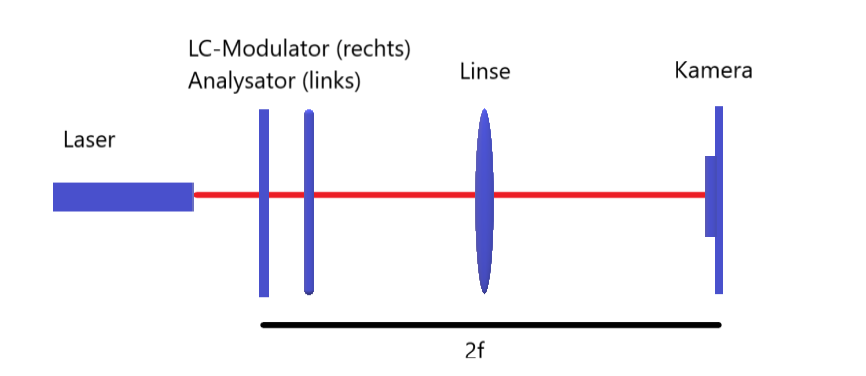
\includegraphics[scale = 1]{Kamera111.png}
	\caption{Aufbau zur Aufnahme von Beugungsbildern, die von dem LC-Modulator erzeugt werden mit Hilfe einer Kamera.}
	\label{423}
\end{figure}
\subsubsection{Auswertung}
In diesem Teil werden Beugungsbilder verschiedener DOE's aufgenommen. Darunter befinden sich der Einzelspalt, der Doppelspalt und das Gitter. Bei dem Einzelspalt werden zwei verschiedene Strukturgrößen benutzt.
\begin{figure}[h!]
	\centering
	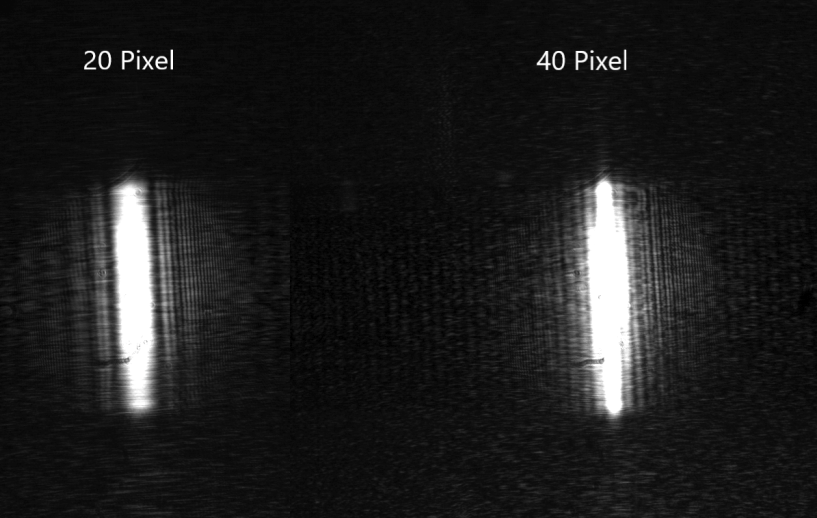
\includegraphics[scale = 1]{pixelverg.png}
	\caption{}
	\label{verg}
\end{figure}

\subsubsection{Unsicherheiten}
\subsubsection{Diskussion}




